Before we dive in into the specifics, we first will showcase the final architecture in the ECS, which is below:

\begin{figure}[!htbp]
    \centering
    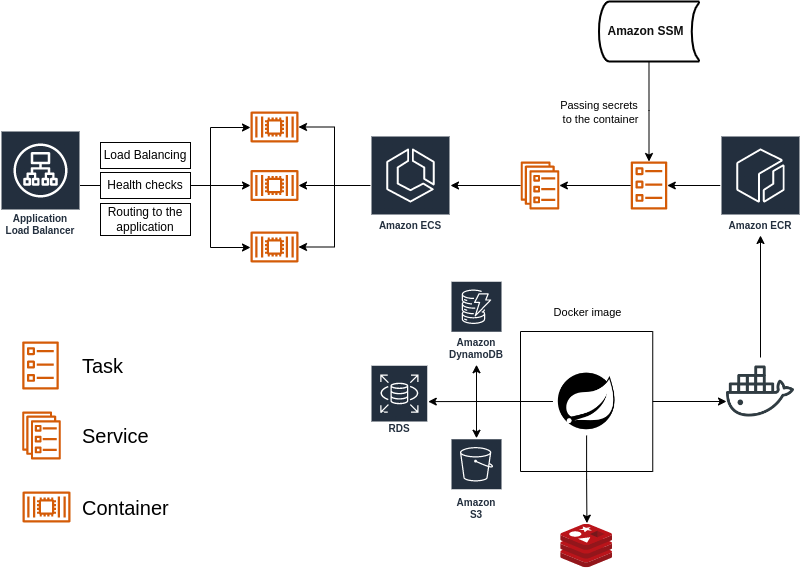
\includegraphics[width=\textwidth]{images/ECS}
    \caption{\footnotesize{ECS Architecture}}
    \label{fig:ECSArch}
\end{figure}

Task: the component which takes care of running the containers.

Service: the component which manages the tasks.

Container: the image that is running on the task.

\subsection {ECS Containerization and secrets}

The ECS solution was a bit of a challenge to get it to work,
as it was a containerized solution, and not a native one.
So the first step was to containerize the solution, and have a safe image 
that doesn't expose any secrets or environment variables.

In the docker way, we can just pass them through the command line,
and the solution will run perfectly.

But here relied a problem that was the ECS solution, it didn't have a simple
way to feed it the credentials, environment variables neither files, so we had to opt
for using the SSM or Secrets Manager
which is yet another hosted solution to store strings as secrets, and then those could be 
passed to the ECS services.

With the Secrets Manager, for the strings secrets it was a simple writing / reading process
to store and retrieve the secrets. But for the files it was a bit more complicated, there
wasn't a direct way to do that.

Finally we came up with the following solution, which is as follows:

\begin{itemize}
    \item Serialize the content of the file into a base64 string
    \item Store the base64 string in the SSM
    \item Pass the SSM secret to the ECS service
    \item Retrieve the secret from the SSM as a environment variable
    \item Decode the base64 string
    \item Store the deserialized base64 in a file in the container
    \item Point an environment variable to the file
\end{itemize}

As such we managed to pass aws credentials, google credentials and Redis Labs credentials.

\subsection {Load Balancer and routing}

As shown in the ECS Architecture, we had a load balancer in front of the running tasks, which has four main goals:

\begin{itemize}
    \item To take care of the incoming traffic from the client side
    \item To ensure that the traffic distributed evenly
    \item To ensure that the tasks are healthy
    \item To ensure that the tasks are not overloaded and manage it's scalability.
\end{itemize}

\begin{figure}[!htbp]
    \centering
    \includegraphics[width=\textwidth]{images/loadBalancer.png}
    \caption{\footnotesize{Load Balancer Interaction with the backend}}
    \label{fig:loadbalancer}
\end{figure}

So the load balancer is as shown in figure \ref{fig:loadbalancer}, it took traffic from
port 80 where it had an exposed dns link, then it routed it through a VPS to the
containers that are exposing post 8080 in their local network, having healthchecks
done on the endpoint /actuator/health .

\newpage

With that set in place, we had pretty much everything setup to start testing for the
load handling by the ecs to check for the health of the containers and the measures
to be set to ensure that the auto scaling is setup with the right parameters.

So first, we written scripts that did kind of overload the server with the requests,
asynchronously deploy the containers and check monitoring metrics.


The script worked as follows:

\begin{figure}[!htbp]
    \centering
    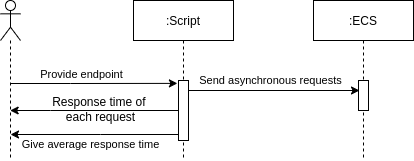
\includegraphics[width=0.7\textwidth]{images/scriptdos.png}
    \caption{\footnotesize{Load Test Script}}
    \label{fig:loadtest}
\end{figure}

So firstly it took the endpoint to be hit, in case it was a private endpoint you'd need to
provide the credentials to. Then put in place the number of requests to be sent and
finally run it.

Once it started running it was a simple case of sending requests asynchronously in fibers
or virtual threads, and then printing the response time of each request, as such we could
monitor the handling time of the requests being affected by the load of requests.

Thus it we could find the right parameters for the auto scaling, based on the number of
requests being sent per second, which at the time of tests was around 1000 request per
second without the response time being affected.

And as most the back-end services relying heavily on the memory, we ensured to put a 70\%
memory usage limit on the containers before spawning new instances to handle the load, in
case of autoscaling by memory.

\subsection{Deployment}

Finally after testing everything, and having deployed one ECS service succesfully, we had
to automate the deployment process, so that we could handle new versions and code update
without much effort.

This came in the form of a gradle task, which was as follows:

    \begin{figure}[!htbp]
        \centering
        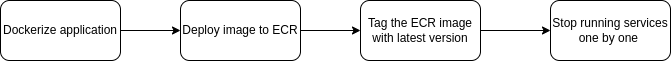
\includegraphics[width=\textwidth]{images/gradle.png}
        \caption{\footnotesize{Gradle Task}}
        \label{fig:gradle}
    \end{figure}

The dockerization part of the gradle task was handled using a third party plugin,
then the deployment to ECR is done using the AWS CLI, by linking the ECR to docker,
then pushing the image is automatically uploaded to ECR.
Once this is done, the ECS service has to handle the update of the image, 
and this was done through a bash script that took in charge of getting a list 
of the running tasks, then stopping one of them, and wait for a new one to spawn 
such as to avoid down time during the update of the service.

For clearer representation of the flow of this task, here's a sequence diagram:

    \begin{figure}[!htbp]
        \centering
        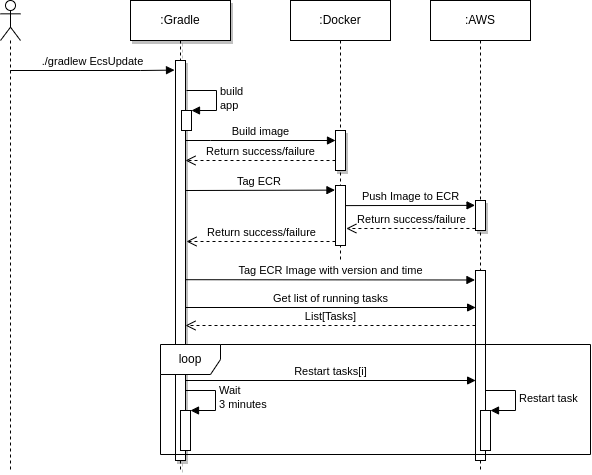
\includegraphics[width=0.9\textwidth]{images/gradleTask.png}
        \caption{\footnotesize{Deployment Sequence Diagram}}
        \label{fig:deployment}
    \end{figure}


